\chapter{CLaRyS prototypes}\label{chap::3}


\vfill

\minitoc

\newpage

\glsresetall


Following the highlighted limits of ion beam therapy (see chapter~\ref{chap::1}), a collaboration of five French research institutions was established in 2008 (??) with the aim of exploring different experimental solutions for the ion range online monitoring. The research group originally involved the \enquote{\gls{ipnl}}, the \enquote{\gls{cppm}}, the \enquote{\gls{lpsc}} in Grenoble, the \enquote{\gls{lpc}} and the \enquote{\gls{creatis}} in Lyon. The collaboration focuses on the investigation of methods and detection solution for the online monitoring of ion beam range during ion beam therapy treatment, and is so called \gls{clarys}.\\
The main goal of the created collaboration is the parallel development of three gamma detection systems to be employed for ion range online monitoring purpose in the ion beam therapy field: a \gls{pet} detector, a multi-collimated gamma camera and a Compton camera.\\ The design and development of the \gls{pet} system is mainly managed by the \gls{lpc} group, which left the collaboration in 2017, and the this detection system is not treated in this thesis work.\\ 
In this chapter the two gamma cameras (multi-collimated and Compton) prototypes are described in details, and the present status of the instrumental development is presented. In the following, an entire chapter (chapter~\ref{chap::6}) is dedicated to the tests of the detectors performed on ion beams. 

\section{CLaRyS gamma camera components}\label{chap3::sec::CLaRyScameras}

The two gamma cameras under development by the CLaRyS collaboration are devoted to the detection of prompt-gamma rays emitted during ion beam treatments (see section~\ref{chap1::sec::PromptGammas}). The design of the two cameras has been optimized by different Monte Carlo simulation studies for what concerns both the detector components and the geometrical setup.\\
As already mentioned, a Compton camera is usually composed of two detector sections, a scatterer and an absorber: the CLaRyS prototype respects the standard design. In the scatterer, described in section~\ref{chap3::subsec::scatterer}, the prompt-gamma incoming ray is deflected by Compton interaction and the interaction position and energy deposited are stored. The scattered photon reaches then the absorber section, where its energy is ideally totally deposited and stored, again with the interaction position. This configuration is used to provide what is usually defined as \enquote{electronic collimation}, but a mechanical collimation is still an option for photon detection and localization. The scatterer section can be replaced by a mechanical collimator, described in section~\ref{chap3::subsec::collimator}, which selects the parallel incoming photons then absorbed by the same absorber detector (a geometrical setup adaptation is possible to optimize the detection performance and will be discussed in the following). The mechanically collimated system is called multi-collimated camera, due to the collimator multi-slit structure.\\ 
As underlined in section~\ref{chap1::sec::background}, the prompt-gamma measurements are affected by several sources of background: in particular, the signals detected by the two cameras can come from secondary particles other then prompt-gammas, like photons from positron annihilation, neutrons and protons (for beam of ions heavier then protons). One of the possible solution for background rejection is the use of \gls{tof} information (see section~\ref{chap1::sec::TOF}), requiring a further detection section dedicated to the beam tagging. A beam tagging hodoscope is being developed in parallel and can be coupled to both the gamma cameras for \gls{tof} measurements; its description is presented in section~\ref{chap3::subsec::hodoscope}.\\
A schematic view of the two prototypes is given in figure~\ref{chap3::fig::camerasScheme}.\\

\begin{figure}
\begin{subfigure}[b]{.5\textwidth}
\centering
\includegraphics[width=1\textwidth]{03_GraphicFiles/chapter3_CLaRySproto/schemes/schema_Collimated_withHodo.pdf}
\caption{Scheme of the multi-collimated camera with the beam tagging hodoscope.}
\label{chap3::subfig::multiCollScheme}
\end{subfigure}
\begin{subfigure}[b]{.5\textwidth}
\centering
\includegraphics[width=1\textwidth]{03_GraphicFiles/chapter3_CLaRySproto/schemes/schema_Compton_withHodo.pdf}	
\caption{Scheme of the Compton camera with the beam tagging hodoscope.}
\label{chap3::subfig::ComptonScheme}
\end{subfigure}
\caption{Schematic view of the two CLaRyS gamma camera prototypes: the multi-collimated camera (top) and the Compton camera (bottom).}
\label{chap3::fig::camerasScheme}
\end{figure}
 

%%%%%%%%%%%%%%%%%%%%%%%%%%%%%%%%%%   SCATTERER  %%%%%%%%%%%%%%%%%%%%%%%%%%%%%%%%%%%%%%%%%%%%

\subsection{Scatterer}\label{chap3::subsec::scatterer} 
The scatterer stack is one of the components of the Compton camera prototype. Dedicated to the photon Compton scattering, its design has been studied to fulfill the camera requirements.\\ 
The Compton events reconstruction strongly relies on the measurement of the energy deposited by the photon in its Compton interaction, mandatory to properly calculate the Compton scattering angle, which is then the aperture of the resulting Compton cone. The camera accuracy is then strictly dependent on the scatterer energy resolution. At the same time, the camera efficiency is dominated by the balance between Compton interaction and photoelectric absorption probability in the scatterer detector.\\
Given the need of at least two interactions for a proper event reconstruction (a Compton scattering in the scatterer section and an ideally complete absorption in the absorber section, described in~\ref{chap3::subsec::absorber}), the material choice and the geometrical configuration play a fundamental role in the camera operation. The setup must be tuned in order to define the better trade-off between Compton and photoelectric interaction probability and to optimize, as mentioned, the detector energy resolution.\\
Knowing that the Compton interaction probability linearly increases with the material atomic number (Z), while the photoelectric absorption depends on Z$^{n}$ with n varying between 4 and 5 according to the photon primary energy~\parencite{Knoll2000}, it is clear that a low Z material is preferred. Considering now the detector energy resolution, it must be noticed that the main parameter affecting the deposited energy detection is the so called \enquote{Doppler spread}. The Compton angle reconstruction formula in equation~\ref{chap1::eq::Compton} neglects the initial recoil electron state, which is considered free or unbound. The Compton energy transfer continuum results affected by the binding energy of the electron, with a relatively increasing effects for decreasing incident photon energy. This effect adds uncertainty on the reconstructed deposited energy, and so in the Compton angle calculation. Given its direct dependence on the recoil electron binding energy, the \enquote{Doppler spread} is reduced for low Z materials. Following the described theoretical considerations, silicon detectors are the most coherent choice. This choice has been verified in simulation, where a silicon scatterer has been compared to competitor materials; the result are included in the Monte Carlo study presented in chapter~\ref{chap::5}.\\
Dedicated Monte Carlo simulation studies have been performed in order to define the most suitable geometrical configuration for the Compton camera, including the scatterer stack~\parencite{Richard2012}. As a trade-off between detection efficiency and total cost, 10 layers were included in the original scatterer design. Concerning the layer size, about 10$\times$10~cm$^{2}$ of active area in the transverse plane have been identified as the most convenient choice, also considering the absorber size (see section~\ref{chap3::subsec::absorber}) and the distances between the detection sections required by the \gls{tof} measurements and imposed by the detector rate acceptance in clinical conditions (see appendix~\ref{chap::appA}). Moving to the layer thickness, its choice is governed by the definition of the camera operation. The \gls{clarys} Compton camera does not aim to track the Compton recoil electron, which must be then absorbed inside the same scatterer layer where the Compton interaction took place. This requirement is necessary to well reconstruct the Compton interaction angle, which needs the whole transferred energy as parameter; in addition to this, a recoil electron escaping the involved detection layer can interact in a different layer causing false coincidences which affect the camera efficiency and imaging accuracy. In order to minimize the recoil electron escape probability, relatively thick detectors are needed.\\
The technological choice of the collaboration was oriented to silicon \glspl{dssd}, provided by the Norwegian company SINTEF. A schematic view of the detector principle is given in figure~\ref{chap3::fig::dssdTHEO}. The silicon crystal is doped with negative (n) and positive (p) charge carriers on the two opposite sides, creating diodes which are then reverse biased. A polarization voltage is applied to the two opposite sides of the crystal, and a depletion region with no free charges is created. A ionizing particle interacting in the depletion region generates electron-hole pairs in number proportional to the deposited energy. The generated charges drift towards anode (electrons) and cathode (holes) and are converted into electrical signals. The read-out is ensured by the implanted strips, which transfer the charges outside the detection region.\\     

\begin{figure}
\begin{subfigure}[t]{.5\textwidth}
\centering
\includegraphics[width=1\textwidth]{03_GraphicFiles/chapter3_CLaRySproto/Scatterer/DSSD_theory_1.pdf}
\caption{Schematic view of a standard \gls{dssd} (from~\cite{Takeda2008}) and sketch of the signal generation.}
\label{chap3::fig::dssdTHEO}
\end{subfigure}
\begin{subfigure}[t]{.5\textwidth}
\centering
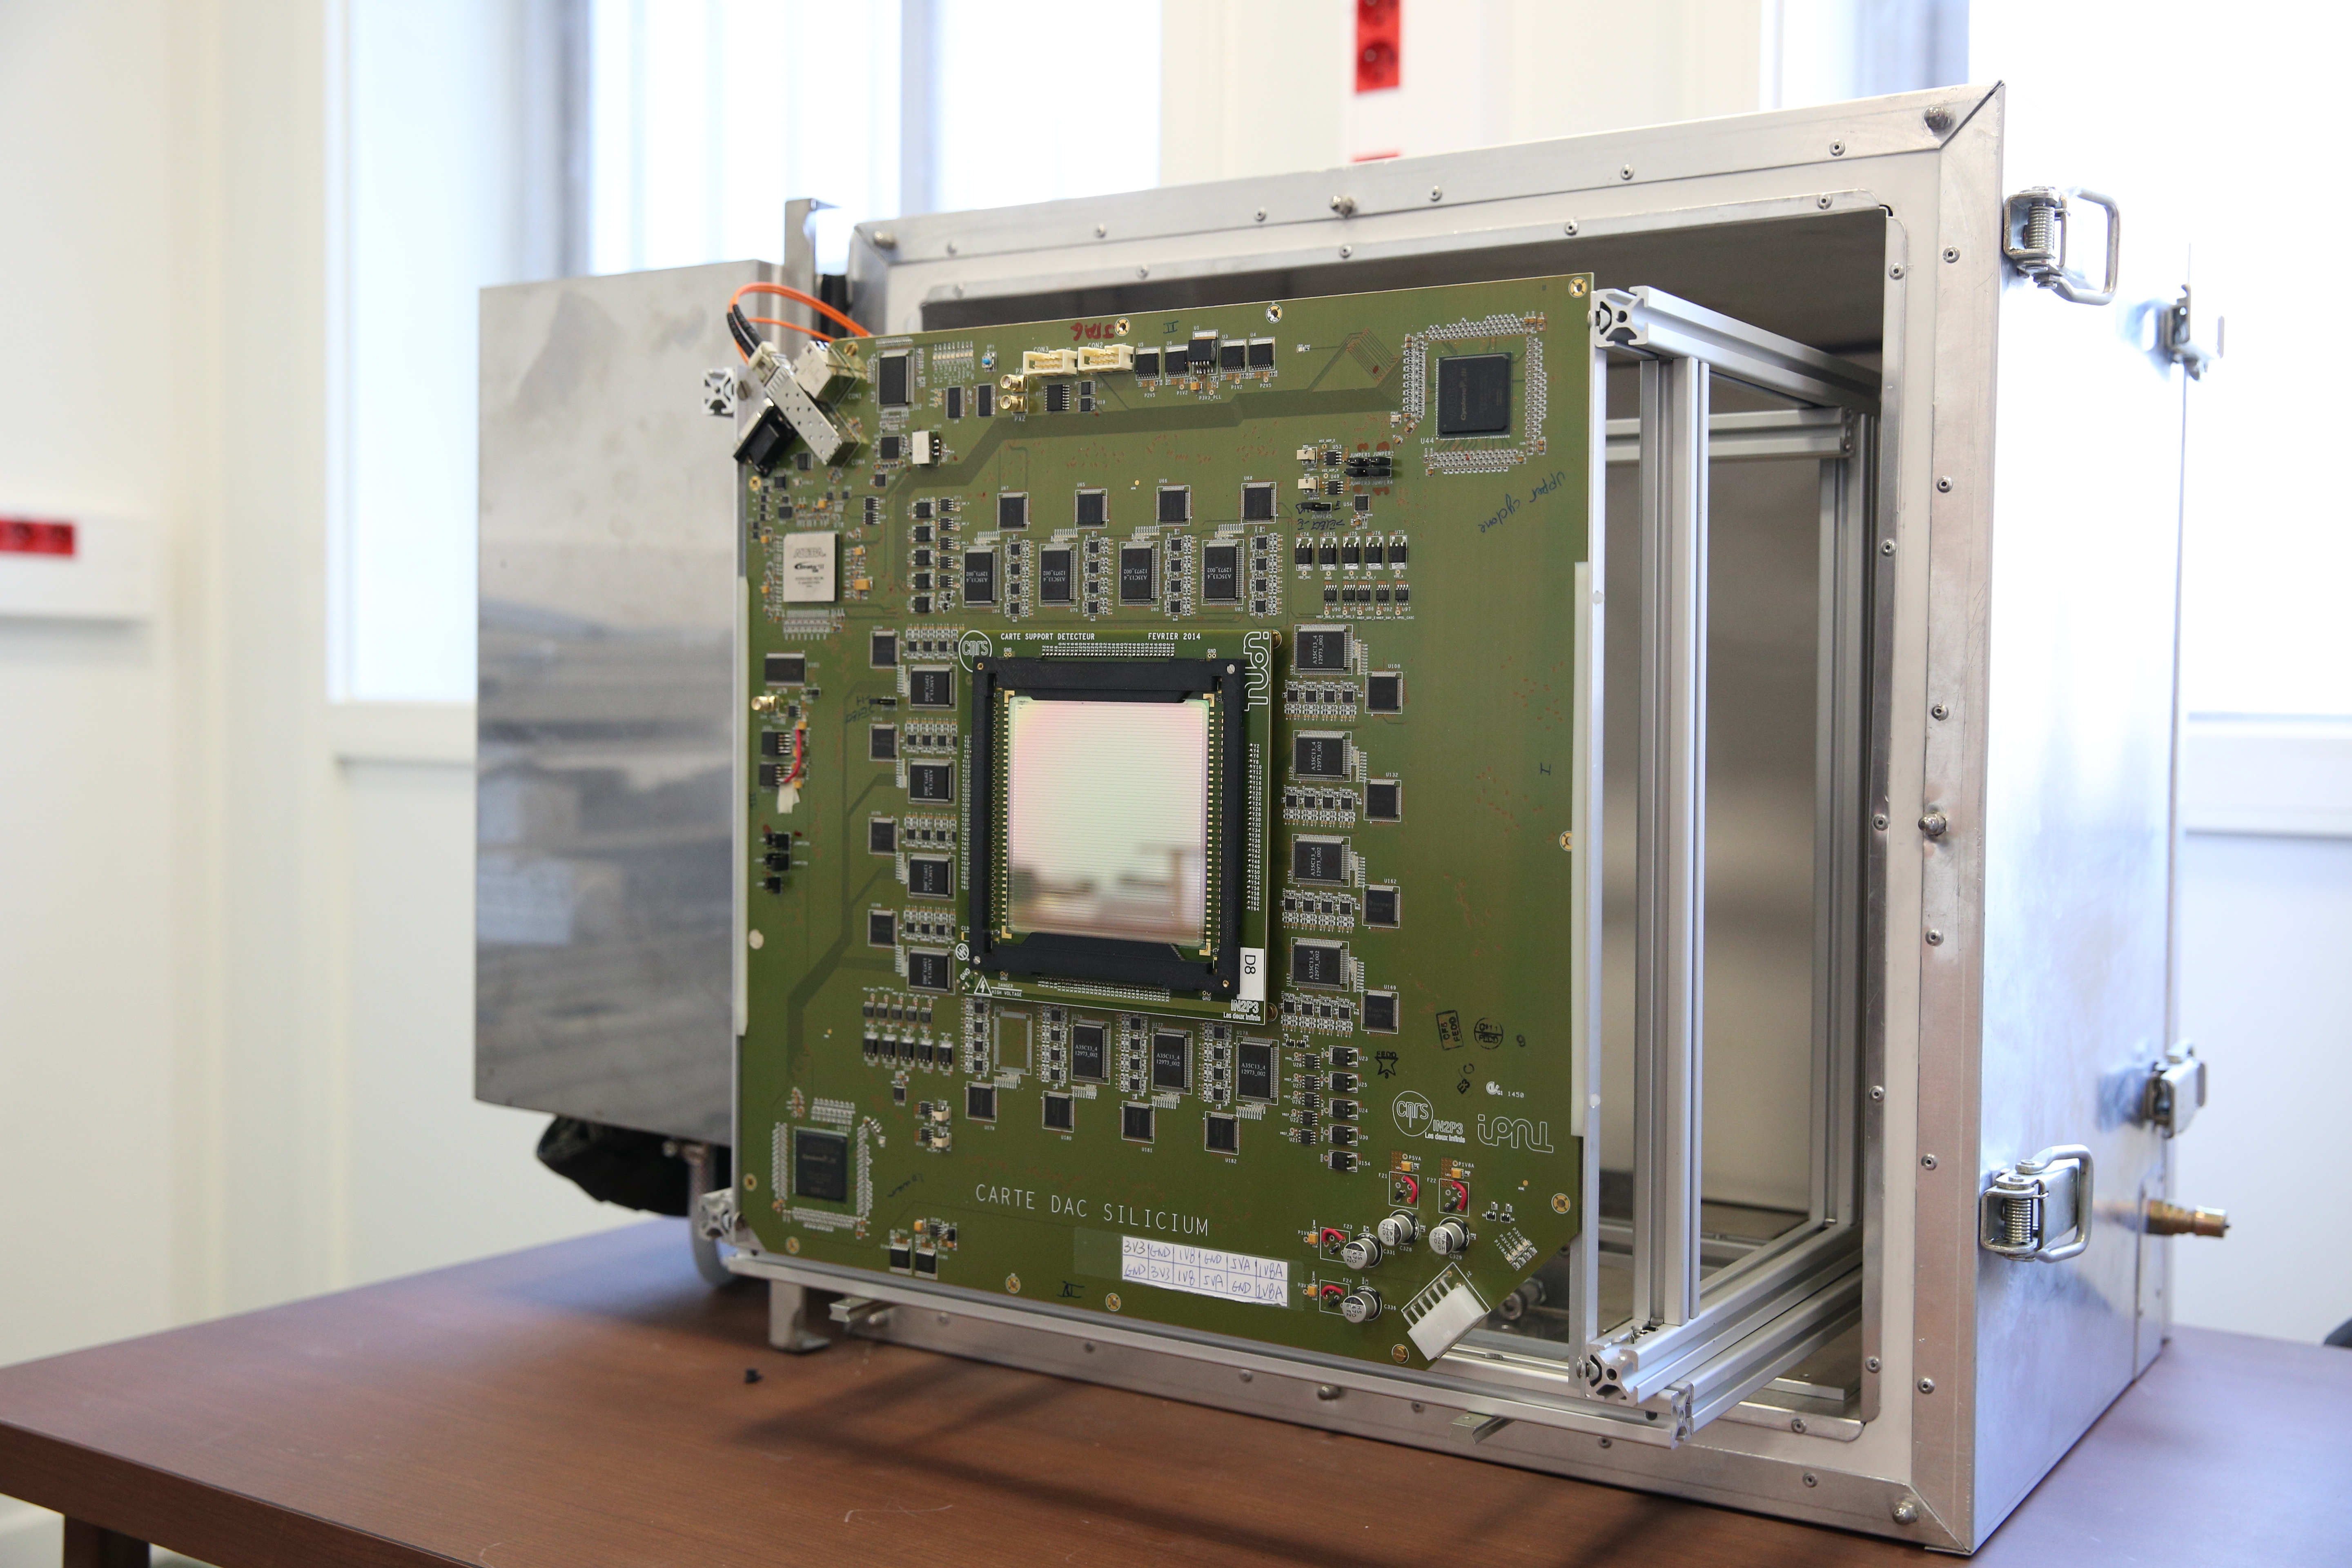
\includegraphics[width=1\textwidth, height=16em]{03_GraphicFiles/chapter3_CLaRySproto/Scatterer/ScattererThermalBox.JPG}
\caption{Scatterer silicon layer with its \gls{fe} card in the thermal regulated box (described in section~\ref{chap3::subsubsec::ScattThermBox}).}
\label{chap3::fig::ScattPicture}
\end{subfigure}
\caption{}
\label{chap3::fig::scatterer}
\end{figure} 

Each layer has an active volume of 96$\times$96$\times$2~mm$^{3}$, segmented with 64 strips per detection plane. The strip pitch is 1.41~mm, for a strip width of 1.31~mm. The applied polarization voltage is nominally -750~V, and it is uniformly shared on the whole surface to obtain a homogeneous depletion region. A guard ring, composed of 23 strips surrounding the read-out ones, ensures the desired voltage gradient. The p and n strips are then connected to the read-out electronics via bonding cables.\\
The \gls{fe} electronics card has been developed by the \gls{ipnl} electronics group and is described in details in section~\ref{chap3::subsubsec::ScattFEcard}. The silicon detector is directly plugged on the card, and the mechanical support for the scatterer stack has been studied according to the card size, as shown in figure~\ref{chap3::fig::ScattPicture}.\\   
Among the 10 received \glspl{dssd}, only 7 fulfilled the requirements imposed by the Compton camera application, mainly in terms of noise level; 3 layer have been rejected, so that the final prototype scatterer is composed of 7 silicon planes.\\
The 7 selected layers have been characterized with a temporary acquisition system in terms of leakage current at different temperatures. The results of these measurements can be found in~\cite{Ley2015}. The measurements allowed to verify the producer specifications in terms of polarization voltage to be applied for a complete detector depletion, as well as to identify the noisy strips and create a complete characterization database. In addition to this, they highlighted the need to cool the detectors down to at least -20~\textdegree{}C in order to reduce the leakage current to acceptable levels, and so reducing the total noise level, affecting the detector performance. In order to accomplish the cooling task and respect, at the same time, the clinical restrictions, a thermal regulated box based on cold air pumps has been designed and produced. It operates as the scatterer stack mechanical support, and it is described in section~\ref{chap3::subsubsec::ScattThermBox}.\\
      
 

\subsubsection{Scatterer Front-End card}\label{chap3::subsubsec::ScattFEcard}

\subsubsection{Scatterer thermal regulated box}\label{chap3::subsubsec::ScattThermBox}



%%%%%%%%%%%%%%%%%%%%%%%%%%%%%%%%%%   COLLIMATOR  %%%%%%%%%%%%%%%%%%%%%%%%%%%%%%%%%%%%%%%%%%%%

\subsection{Collimator}\label{chap3::subsec::collimator}
 
The multi-collimated camera is equipped with a multi-slit collimator, with tungsten slabs. Its design has been extensively studied in Monte Carlo simulations~\parencite{Pinto2014}, and it can be easily adapted to different geometrical configurations of the absorber detector and to various monitoring requirements. In particular, the distance between neighboring slabs can be modified, as well as the number of total slabs, in order to find the best trade-off between detection efficiency and spatial resolution; this depends on the distance patient-collimator, on the required extension of the field of view and on the desired monitoring time. Two identical collimators of 30$\times$14$\times$17~cm$^{3}$ have been produced, in order to be able to set several absorber configurations in the transverse direction (extended version along the beam axis or in the perpendicular direction). In figure~\ref{chap3::fig::collimatorPicture} a picture of the tungsten collimator is presented.\\

\begin{figure} [!h]
\centering
\includegraphics[width=0.7\textwidth]{03_GraphicFiles/chapter3_CLaRySproto/Collimator/Collimator.pdf}
\caption{Picture of the multi-slit tungsten collimator.}
\label{chap3::fig::collimatorPicture}
\end{figure} 


%%%%%%%%%%%%%%%%%%%%%%%%%%%%%%%%%%   ABSORBER  %%%%%%%%%%%%%%%%%%%%%%%%%%%%%%%%%%%%%%%%%%%%

\subsection{Absorber}\label{chap3::subsec::absorber}

The Compton and multi-collimated camera absorber was initially conceived as a very large surface plane composed of 96 \gls{bgo} blocks recovered from a dismantled \gls{pet} system HR+ by SIEMENS, documented in~\parencite{Adam1997, Brix1997}.\\ 
%%%From BGO paper %%%%%%%%
\gls{bgo} is one of the most used scintillators for gamma detection applications, thanks to a good energy resolution and a optimal gamma detection efficiency. Moreover, the absence of internal radioactivity which characterizes other scintillator materials employed in the same field (i.e.~\gls{lyso}, \gls{lso}), makes it suitable for low noise detectors, required by a Compton camera to reduce the amount of random coincidences, one of the main sources of background for the application in ion beam therapy monitoring~\parencite{Ortega2015}. As highlighted in~\parencite{HuesoGonzalez2015}, \gls{lyso} and \gls{lso} show overall better performances with respect to \gls{bgo} for what concerns energy, time and spatial resolution, due to an about 4 times higher light yield, but the gap is reduced for the detection of gamma rays in the prompt-gamma energy range (especially beyond 1~MeV). The limited cost of \gls{bgo} with respect to \gls{lso} and the comparable performances in the prompt-gamma energy range make it an optimal solution for prompt-gamma camera prototypes.\\
Each \gls{bgo} block has a surface of 3.5$\times$3.8~cm$^2$, with a thickness of 3.0~cm. The mono-block \gls{bgo} crystal is streaked in a 8$\times$8 pseudo-pixel matrix; a reflecting material is inserted between the pseudo-pixels to improve the light collection and optimize the spatial information accuracy via pixel separation. The read-out is achieved via four \gls{pm} tubes per block, composing a quartet, coupled to the block back surface. Thanks to the internal streaked structure of the block, the scintillation light is shared on the four PMs depending on the pseudo-pixel where the interaction takes place (in case of multiple interactions more than 1 pseudo-pixel can be involved). The reconstruction of the position of interaction is done via Anger logic, i.e.~with a center of gravity calculation.\\
The whole set of recovered blocks was supposed to undergo a \enquote{reconditioning} process, including the \gls{pm} removal, the crystal back surface polishing with diamond-based abrasive tool, the single \glspl{pm} gain characterization and grouping in quartets with similar gains, the final re-coupling of the \glspl{pm} and block shielding.\\ A set of \enquote{reconditioned} blocks have been tested with the method described in section~\ref{chap3::sec::charMeasurements} and their performance have been compared to a set of original blocks. An overall degradation of the detection performance has been verified on all the tested \enquote{reconditioned} blocks, which showed lower amplitude output signals probably link to a reduction of the collected scintillation light. Various correction methods have been tested, with unsatisfactory results. According to the outcome of these tests, summarized in~\cite{Sandjong2017}, the collaboration finally opted to adapt the camera design for the use of original, \enquote{non-reconditioned} \gls{bgo} blocks.\\    
Thirty original blocks are now available to compose the absorber detector. In addition to the already presented features, it must be noticed that the lateral surfaces of the original blocks, as well as the half of the \gls{pm} length, are covered by a reflecting material which ensures the complete collection of the scintillation light. This is probably a component which was not well reproduced during the reconditioning process. The whole structure is then protected by a 1~mm thick aluminum foil, which also isolates from external light contamination.\\
Figure~\ref{chap3::fig::block_noPM} shows one \gls{bgo} block before the coupling to the \gls{pm} quartet: the streaked structure is clearly visible, as well as the white reflecting material separating the pseudo-pixels and the one surrounding the block lateral sides. As mentioned, the same material also covers part of the photo-multiplier tubes, as shown in picture~\ref{chap3::fig::originalBlock_noAl}, where the four \glspl{pm} are glued to the block back surface. The described aluminum cover is visible in figure~\ref{chap3::fig::originalBlock_withAl}, while in figure~\ref{chap3::fig::BGOblockScheme} a scheme of a block together with the related \gsl{pm} quartet is given. The spatial reconstruction logic is also reported in the same figure. To be noticed that the streaked structure of the pseudo-pixels depends on their position in the block: the reflecting streak covers about three fourth of the block thickness for the for the lateral pseudo-pixels, while it is limited to half of the block thickness for the central ones.\\ 

\begin{figure}
\begin{subfigure}[b]{.5\textwidth}
\centering
\includegraphics[width=1\textwidth, height=16em]{03_GraphicFiles/chapter3_CLaRySproto/Absorber/images/block_noPM}
\caption{BGO raw block.}
\label{chap3::fig::block_noPM}
\end{subfigure}
\begin{subfigure}[b]{.5\textwidth}
\centering
\includegraphics[width=1\textwidth, height=16em]{03_GraphicFiles/chapter3_CLaRySproto/Absorber/images/originalBlock_noAluminum}
\caption{BGO crystal coupled to PM quartet.}
\label{chap3::fig::originalBlock_noAl}
\end{subfigure}
\begin{subfigure}[b]{.5\textwidth}
\centering
\includegraphics[width=1\textwidth, height=16em]{03_GraphicFiles/chapter3_CLaRySproto/Absorber/images/originalBlock_withAluminum}
\caption{BGO complete module with aluminum cover.}
\label{chap3::fig::originalBlock_withAl}
\end{subfigure}
\begin{subfigure}[b]{.5\textwidth}
\centering
\includegraphics[width=1\textwidth, height=16em]{03_GraphicFiles/chapter3_CLaRySproto/Absorber/block_scheme.pdf}
\caption{Scheme of a \gls{bgo} block and its spatial reconstruction logic.}
\label{chap3::fig::BGOblockScheme} 
\end{subfigure}
\caption{Absorber modules.}
\label{chap5::fig::BGO_block}
\end{figure}


\subsubsection{Absorber Front-End and read-out cards}\label{chap3::subsubsec::AbsorberFEcard}


A custom front-end card has been designed and produced by the \gls{lpc} research group and is used for the read-out of each \gls{bgo} block. The card is equipped with four voltage modulators which divide the provided high voltage on the 4 photo multiplier tubes. The voltage sent to each PM can be mechanically tuned via screw-potentiometers on these modules. The card is equipped with differential output channels, through which the \gls{pm} signals are sent to the read-out card, called ASM card. A picture of the \gls{fe} card is given in figure~\ref{chap3::fig::FEcard}. To be noticed that 4 analog output channels has been added on some cards in order to allow laboratory tests with a signal treatment based on standard electronics modules, as described in section~\ref{chap3::sec::charMeasurements}. 

\begin{figure}
\begin{subfigure}[b]{.5\textwidth}
\centering
\includegraphics[width=1\textwidth]{03_GraphicFiles/chapter3_CLaRySproto/Absorber/images/FEcard}
\caption{Front-End card of the absorber BGO detectors.}
\label{chap3::fig::FEcard} 
\end{subfigure}
\begin{subfigure}[b]{.5\textwidth}
\centering
\includegraphics[width=1\textwidth]{03_GraphicFiles/chapter3_CLaRySproto/Absorber/ASMcard.pdf}
\caption{ASM card of the absorber BGO detectors.}
\label{chap3::fig::ASMcard} 
\end{subfigure}
\caption{}
\label{chap5::fig::AbsorberCards}
\end{figure}

DESCRIPTION OF THE ASM CARD

\subsubsection{Absorber mechanical support}\label{chap3::subsubsec::AbsorberMechanics}

A first mechanical structure for the absorber detector was initially conceived by the \gls{lpc} group in order to hold up to 100 modules, foreseen by the original camera design. The reduction of the number of available blocks caused by the \enquote{reconditioning} process failure make necessary an adaptation of such a support. The new design has been carried out by the mechanics group of the \gls{ipnl} in order to be compact and flexible in terms of detection modules setup. Figure~\ref{chap3::fig::absorber_scheme} displays both a picture and a scheme of the absorber configuration with its mechanical support. The two lateral sides are built with \gls{pmma} boards connected by metal bars, and the \gls{bgo} blocks can be arranged in up to 5 rows of variable size, ranging from 3 to 7 blocks. Each block row is supported by a thin metal foil, designed to reduce at minimum the blocks separation and to respect the original ring geometry deriving from the SIEMENS \gls{pet} system. The blocks composing a row are then laterally pressed via two screws on the two sides of the structure, which can also be used to adapt the rows relative position horizontally. On the back side, a metal bar is added to avoid undesired movements, and the \gls{fe} cards are fixed with plastic pillars. The realized support results to be versatile, compact and adapted to the prototype tests for both the Compton camera (where a squared setup is preferred) and the multi-collimated one (where the collimator geometry must be fit by the absorber geometrical configuration).       

\begin{figure}
\begin{subfigure}[b]{.5\textwidth}
\centering
\includegraphics[width=1\textwidth, height=16em]{03_GraphicFiles/chapter3_CLaRySproto/Absorber/images/absorber_picture.JPG}
\caption{Picture of the absorber detector in its mechanical support.}
\label{chap3::fig::absorberPicture}
\end{subfigure}
\begin{subfigure}[b]{.5\textwidth}
\includegraphics[width=1\textwidth, height=16em]{03_GraphicFiles/chapter3_CLaRySproto/Absorber/images/Absorbeur.jpg}
\caption{Scheme of the absorber detector with its mechanical support.}
\label{chap3::fig::absorber30Scheme}
\end{subfigure}
\caption{Absorber front view with the BGO block lines arranged in the mechanical support (left). Scheme of the BGO absorber with its mechanical support (right).}
\label{chap3::fig::absorber_scheme}
\end{figure}

%%%%%%%%%%%%%%%%%%%%%%%%%%%%%%%%%%   HODOSCOPE  %%%%%%%%%%%%%%%%%%%%%%%%%%%%%%%%%%%%%%%%%%%%

\subsection{Beam tagging hodoscope}\label{chap3::subsec::hodoscope}

A beam tagging hodoscope is being developed in parallel to the two gamma cameras, mainly for background rejection and reconstruction optimization purposes [CIT]. As already mentioned, the detection of prompt-gammas (with mechanical or \enquote{electronical} collimation), is affected by the presence of other secondary particles produced during the ion beam irradiation, mainly neutrons. This background source can be efficiently identified and removed my applying \gls{tof} selection windows to the data acquisition. The \gls{tof} measurements can be performed using the accelerator radio-frequency signal as reference, but a direct beam detection results to be more accurate. An auxiliary detector is then needed before the beam interaction in the patient.\\ 
The \gls{clarys} hodoscope prototype is designed to provide space and time information about the incoming primary beam, particle by particle or bunch by bunch, depending on the beam intensity and detector efficiency and rate acceptance which must be characterized. In addition to the already explained use of the time information, a space primary particle tagging can be used to improve the reconstruction accuracy and constraint the possible reconstructed emission vertex in case of analytic reconstruction approach for both the multi-collimated and Compton cameras (see chapter~\ref{chap::2}).\\  
The detector under development is based on squared 1~mm$^{2}$ polystyrene scintillating fibers BCF-12, 140~mm in length, provided by Saint Gobain~\parencite{SaintGobain2017}. A picture of the hodoscope on its mechanical support (detailed in the following) is presented in figure~\ref{chap3::fig::HodoscopeMain}. The fibers are arranged into two perpendicular planes for a two-dimensional spatial information: each plane is composed of 128 fibers, for a total active area (for 2D measurements in coincidence) of 128$\times$128~mm$^{2}$. The active detector surface is completely covered with black reflective tape, which shields from external light. The scintillation light produced in the fibers by a ionizing particle deposing energy is transported to the read-out system via FORETEC optical fibers (1.55~cm diameter, 1~m length), which are connected to the scintillating fibers thanks to a custom mechanical support and to a proper gluing process (see figure~\ref{chap3::fig::HodoMounting}). Each scintillating fibers is read-out on both sides to optimize the detector efficiency and improve the time resolution which is not depending on the interaction position along the fiber with this configuration, so that the total number of read-out channels is 512. The signal read-out is ensured by 8 multi-anode \glspl{pm} Hamamatsu H8500~\parencite{Hamamatsu2006} shown in figure~\ref{chap3::fig::PMH8500}. The optical fibers are connected to the \gls{pm} anode surfaces through a plastic custom mask, shown in figure~\ref{chap3::fig::PMmask}. The \glspl{pm} are equipped with custom black boxes which operate as mechanical support and external light protection (see figure~\ref{chap3::fig::HodoMounting}). In order to provide further light isolation, the whole \gls{pm} boxes are covered with black tape.\\
The optical fibers are connected to the \glspl{pm} with the aim of increasing the maximum counting rate. 4 \glspl{pm} are dedicated to the read-out of the horizontal fibers, and 4 to the vertical ones, and the neighboring fibers are connected to different \glspl{pm}. An active area of 4$\times$4~mm$^{2}$ on the two planes is then read-out by all the 8 \glspl{pm}. Moreover, the two sides of the same scintillating fiber are connected on the same \gls{pm}. This fiber connection logic also improve the detector robustness; in case of problem on one \gls{pm}, only 1~mm each 4~mm is lost on a single plane, so that the detection of the beam is still possible on the whole active area.\\  
Each \gls{PM} is connected to a single custom \gls{fe} card. The hodoscope \gls{fe} cards have been developed by the \gls{ipnl} electronics group: their design is described in section~\ref{chap3::subsubsec::HodoFEcard}. 8 \gls{fe} cards are then used for the read-out, and the collected data are sent to the acquisition system described in section~\ref{chap3::subsec::cameraElectronicsDAQ}.

\begin{figure}[!htbp]
\centering
\includegraphics[width=0.6\textwidth]{03_GraphicFiles/chapter3_CLaRySproto/Hodoscope/Hodoscope_onTable.jpg}
\caption{\gls{clarys} scintillating fiber hodoscope on its 2-dimensional moving table.}
\label{chap3::fig::HodoscopeMain}
\end{figure}

\begin{figure}
\begin{subfigure}[t]{0.5\textwidth}
\centering
\includegraphics[width=1\textwidth]{03_GraphicFiles/chapter3_CLaRySproto/Hodoscope/Hodoscope_mounting.jpg}
\caption{Scintillating fiber hodoscope during mounting process.}
\label{chap3::fig::HodoMounting}
\end{subfigure}
\begin{subfigure}[t]{0.5\textwidth}
\centering
\includegraphics[width=1\textwidth]{03_GraphicFiles/chapter3_CLaRySproto/Hodoscope/hodoPMfiberConnection.pdf}
\caption{Scheme of the scintillating fiber connection to the \glspl{pm} (top) and of the double-sided fiber read-out (bottom).}
\label{chap3::fig::HodoPMfiberConn}
\end{subfigure}
\newline
\begin{subfigure}[t]{0.5\textwidth}
\centering
\includegraphics[width=1\textwidth, height=5.5cm]{03_GraphicFiles/chapter3_CLaRySproto/Hodoscope/H8500.png}
\caption{Hodoscope read-out \glspl{pm} Hamamatsu H8500.}
\label{chap3::fig::PMH8500}
\end{subfigure}
\begin{subfigure}[t]{.5\textwidth}
\includegraphics[width=1\textwidth, height=5.5cm]{03_GraphicFiles/chapter3_CLaRySproto/Hodoscope/Hodoscope_PMmask.JPG}
\caption{\gls{pm} plastic mask for optical fiber connection.}
\label{chap3::fig::PMmask}
\end{subfigure}
\caption{Details of the \gls{clarys} scintillating fiber hodoscope setup.}
\label{chap3::fig::HodoscopeParts}
\end{figure}


\subsubsection{Hodoscope Front-End card}\label{chap3::subsubsec::HodoFEcard}

The hodoscope is designed to tag in space and time the incoming beam ions, so that the signal read-out must be optimized to provide accurate time measurements and an high detection rate acceptance, with reduced dead time and detection efficiency close to 100\%. In particular, the design requirements include a maximum counting rate acceptance of 10$^{8}$~Hz per detection plane, with a time resolution of 1~ns~\parencite{Krimmer2014}.  The hodoscope \gls{fe} card shown in figure~\ref{chap3::fig::HodoscopeFEcard} has been developed by the \gls{ipnl} electronics group to fulfill the listed requirements. The Hamamatsu \gls{pm} is connected to the 64-channel connector (4 connectors of 16 channels each) and two custom \glspl{asic} are dedicated to the data first treatment (32 channels each).        
 
\begin{figure}
\begin{subfigure}[t]{.3\textwidth}
\centering
\includegraphics[width=1\textwidth]{03_GraphicFiles/chapter3_CLaRySproto/Hodoscope/HodoCard1.jpg}
\caption{Hodoscope Front-End card.}
\label{chap3::fig::HodoscopeFEcard}
\end{subfigure}
\begin{subfigure}[t]{.7\textwidth}
\includegraphics[width=1\textwidth]{03_GraphicFiles/chapter3_CLaRySproto/Hodoscope/HodoCardDesign.pdf}
\caption{Hodoscope Front-End card detailed design.}
\label{chap3::fig::HodoscopeFEcardDesign}
\end{subfigure}
\caption{Hodoscope Front-End card developed at \gls{ipnl}.}
\label{chap3::fig::HodoPic}
\end{figure}


CARD DESCRIPTION \parencite{Deng2012, Deng2013}.

\subsubsection{Hodoscope mechanical support}\label{chap3::subsubsec::HodoMechanics}

The beam tagging hodoscope is set between the beam nozzle and the patient and it requires a dedicated mechanical support. In order to profit of the large active area and to be able to remotely control the hodoscope position in the beam transverse plane, the detector is mounted on a 2-dimensional moving table (see the picture in figure~\ref{chap3::fig::HodoscopeMain}), which also supports the \gls{fe} cards. Detector and \gls{fe} cards are then integral and translate together. A scheme of the moving table is given in figure~\ref{chap3::fig::HodoscopeSchemeMech}.\\
   
\begin{figure}[!htbp]
\centering
\includegraphics[width=0.5\textwidth]{03_GraphicFiles/chapter3_CLaRySproto/Hodoscope/HodoScheme.png}
\caption{Hodoscope mechanical support scheme.}
\label{chap3::fig::HodoscopeSchemeMech}
\end{figure}

The 2-axis table is provided by Beijing Winner Optical Instruments; it is composed of two motorized linear stages, connected via a right angle bracket. The two stages have a moving range of 30~cm each and the stepper motors have a step resolution of 20~\charmum. The employed motor controller is a Newport XPS-Q8~\parencite{Newport2017}, equipped with 8 channels for the simultaneous control of a maximum of 8 motors. The movements are steered with an online interface or with a LabVIEW based program, which will be integrated in the final setup of the slow control software under development with the cameras.

\subsubsection{Small hodoscope prototypes}\label{chap3::subsubsec::SmallHodoProto}
Before the production of the large active surface hodoscope prototype described in section~\ref{chap3::subsec::hodoscope}, two smaller prototypes have been produced and tested in order to assess the potential of such a kind of detector for the required application. The first and simplest version consisted of one single scintillating fiber per plane, and the readout was performed with two \gls{pm} tubes directly coupled to the scintillating fibers, without optical fibers. A picture of this prototype is given in figure~\ref{chap3::fig::singleFibHodo}. This simple version of the detector has been used as a demonstrator of the basic detection principle.\\ 

\begin{figure}
\begin{subfigure}[t]{.5\textwidth}
\includegraphics[width=0.8\textwidth]{03_GraphicFiles/chapter3_CLaRySproto/Hodoscope/hodo2.jpg}
\caption{Hodoscope small prototype, 1$\times$1 scintillating fibers.}
\label{chap3::fig::singleFibHodo}
\end{subfigure}
\begin{subfigure}[t]{.5\textwidth}
\centering
\includegraphics[width=0.8\textwidth]{03_GraphicFiles/chapter3_CLaRySproto/Hodoscope/hodo32_withCard.jpg}
\caption{Hodoscope small prototype, 32$\times$32 scintillating fibers.}
\label{chap3::fig::Hodoscope32}
\end{subfigure}
\caption{Hodoscope small prototypes.}
\label{chap3::fig::HodoSmall}
\end{figure}

A second small size version of the final detector has been produced with almost the same features as the large area prototype but with simplified read-out logic. It is equipped with two perpendicular planes of 32 1~mm$^{2}$ scintillating fibers each (Saint Gobain BCF-10~\parencite{SaintGobain2017}), with a length of 4~cm and a total active area for a 2D read-out of 32$\times$32~mm$^{2}$. As in the big hodoscope, the scintillating fibers are coupled to FORETEC optical fibers which transfer the scintillation light to 4 Hamamatsu H8500 \glspl{pm}. 16 channels per \gls{pm} are used, so that 2 \glspl{pm} are dedicated to the horizontal fibers and 2 to the vertical ones, and the signal read-out is performed on a single side of the scintillating fibers. As the total number of read-out channels is 64, a single \gls{fe} card is enough for the whole detector. In figure~\ref{chap3::fig::Hodoscope32} the 32$\times$32-fiber hodoscope prototype is shown together with its \gls{fe} card; 4 connections cables (16 channels each) are used to couple the \glspl{pm} to the \gls{fe} card.\\
The 32$\times$32-fiber hodoscope prototype has been tested in 2014 on proton and carbon ion beams (at the \gls{ganil} - 75~MeV/u $^{13}$C, \gls{hit} - protons and carbon ions at various energy, \gls{ipno} - 25~MeV protons) with the first version of the \gls{fe} card (see section~\ref{chap3::subsubsec::HodoFEcard}): an efficiency of more than 90\% has been retrieved, with a time resolution of 1~ns \gls{fwhm} (timing measurements performed with respect to the accelerator high frequency signal). Some more details about this beam tests results are given in chapter~\ref{chap::6}. The final version of the \gls{fe} card has been also tested with this detector, and the test description and results are presented in chapter~\ref{chap::6}.  
   

%%%%%%%%%%%%%%%%%%%%%%%%%%%%%%%%%%   ELECTRONICS/DAQ  %%%%%%%%%%%%%%%%%%%%%%%%%%%%%%%%%%%%%%%%%%%%

\subsection{Camera electronics and acquisition system}\label{chap3::subsec::cameraElectronicsDAQ}

\begin{figure}
\begin{subfigure}[t]{.5\textwidth}
\includegraphics[width=0.8\textwidth]{03_GraphicFiles/chapter3_CLaRySproto/Electronics_Acquisition/uTCAcrate_1.jpg}
\caption{}
\label{chap3::fig::uTCAcrate}
\end{subfigure}
\begin{subfigure}[t]{.5\textwidth}
\centering
\includegraphics[width=0.8\textwidth]{03_GraphicFiles/chapter3_CLaRySproto/Electronics_Acquisition/AMC40.jpg}
\caption{}
\label{chap3::fig::AMC40}
\end{subfigure}
\caption{}
\label{chap3::fig::AcquisitionSystem}
\end{figure}

%%%%%%%%%%%%%%%%%%%%%%%%%%%%%%%%%%   MECHANICAL SUPPORT  %%%%%%%%%%%%%%%%%%%%%%%%%%%%%%%%%%%%%%%%%%%%

\subsection{Camera integration and mechanical support}\label{chap3::subsec::CameraMechanics}

\begin{figure}
\begin{subfigure}[t]{.5\textwidth}
\includegraphics[width=0.8\textwidth]{03_GraphicFiles/chapter3_CLaRySproto/Mechanics/TableCameraSchemeBlue.jpg}
\caption{}
\label{chap3::fig::schemeTable}
\end{subfigure}
\begin{subfigure}[t]{.5\textwidth}
\centering
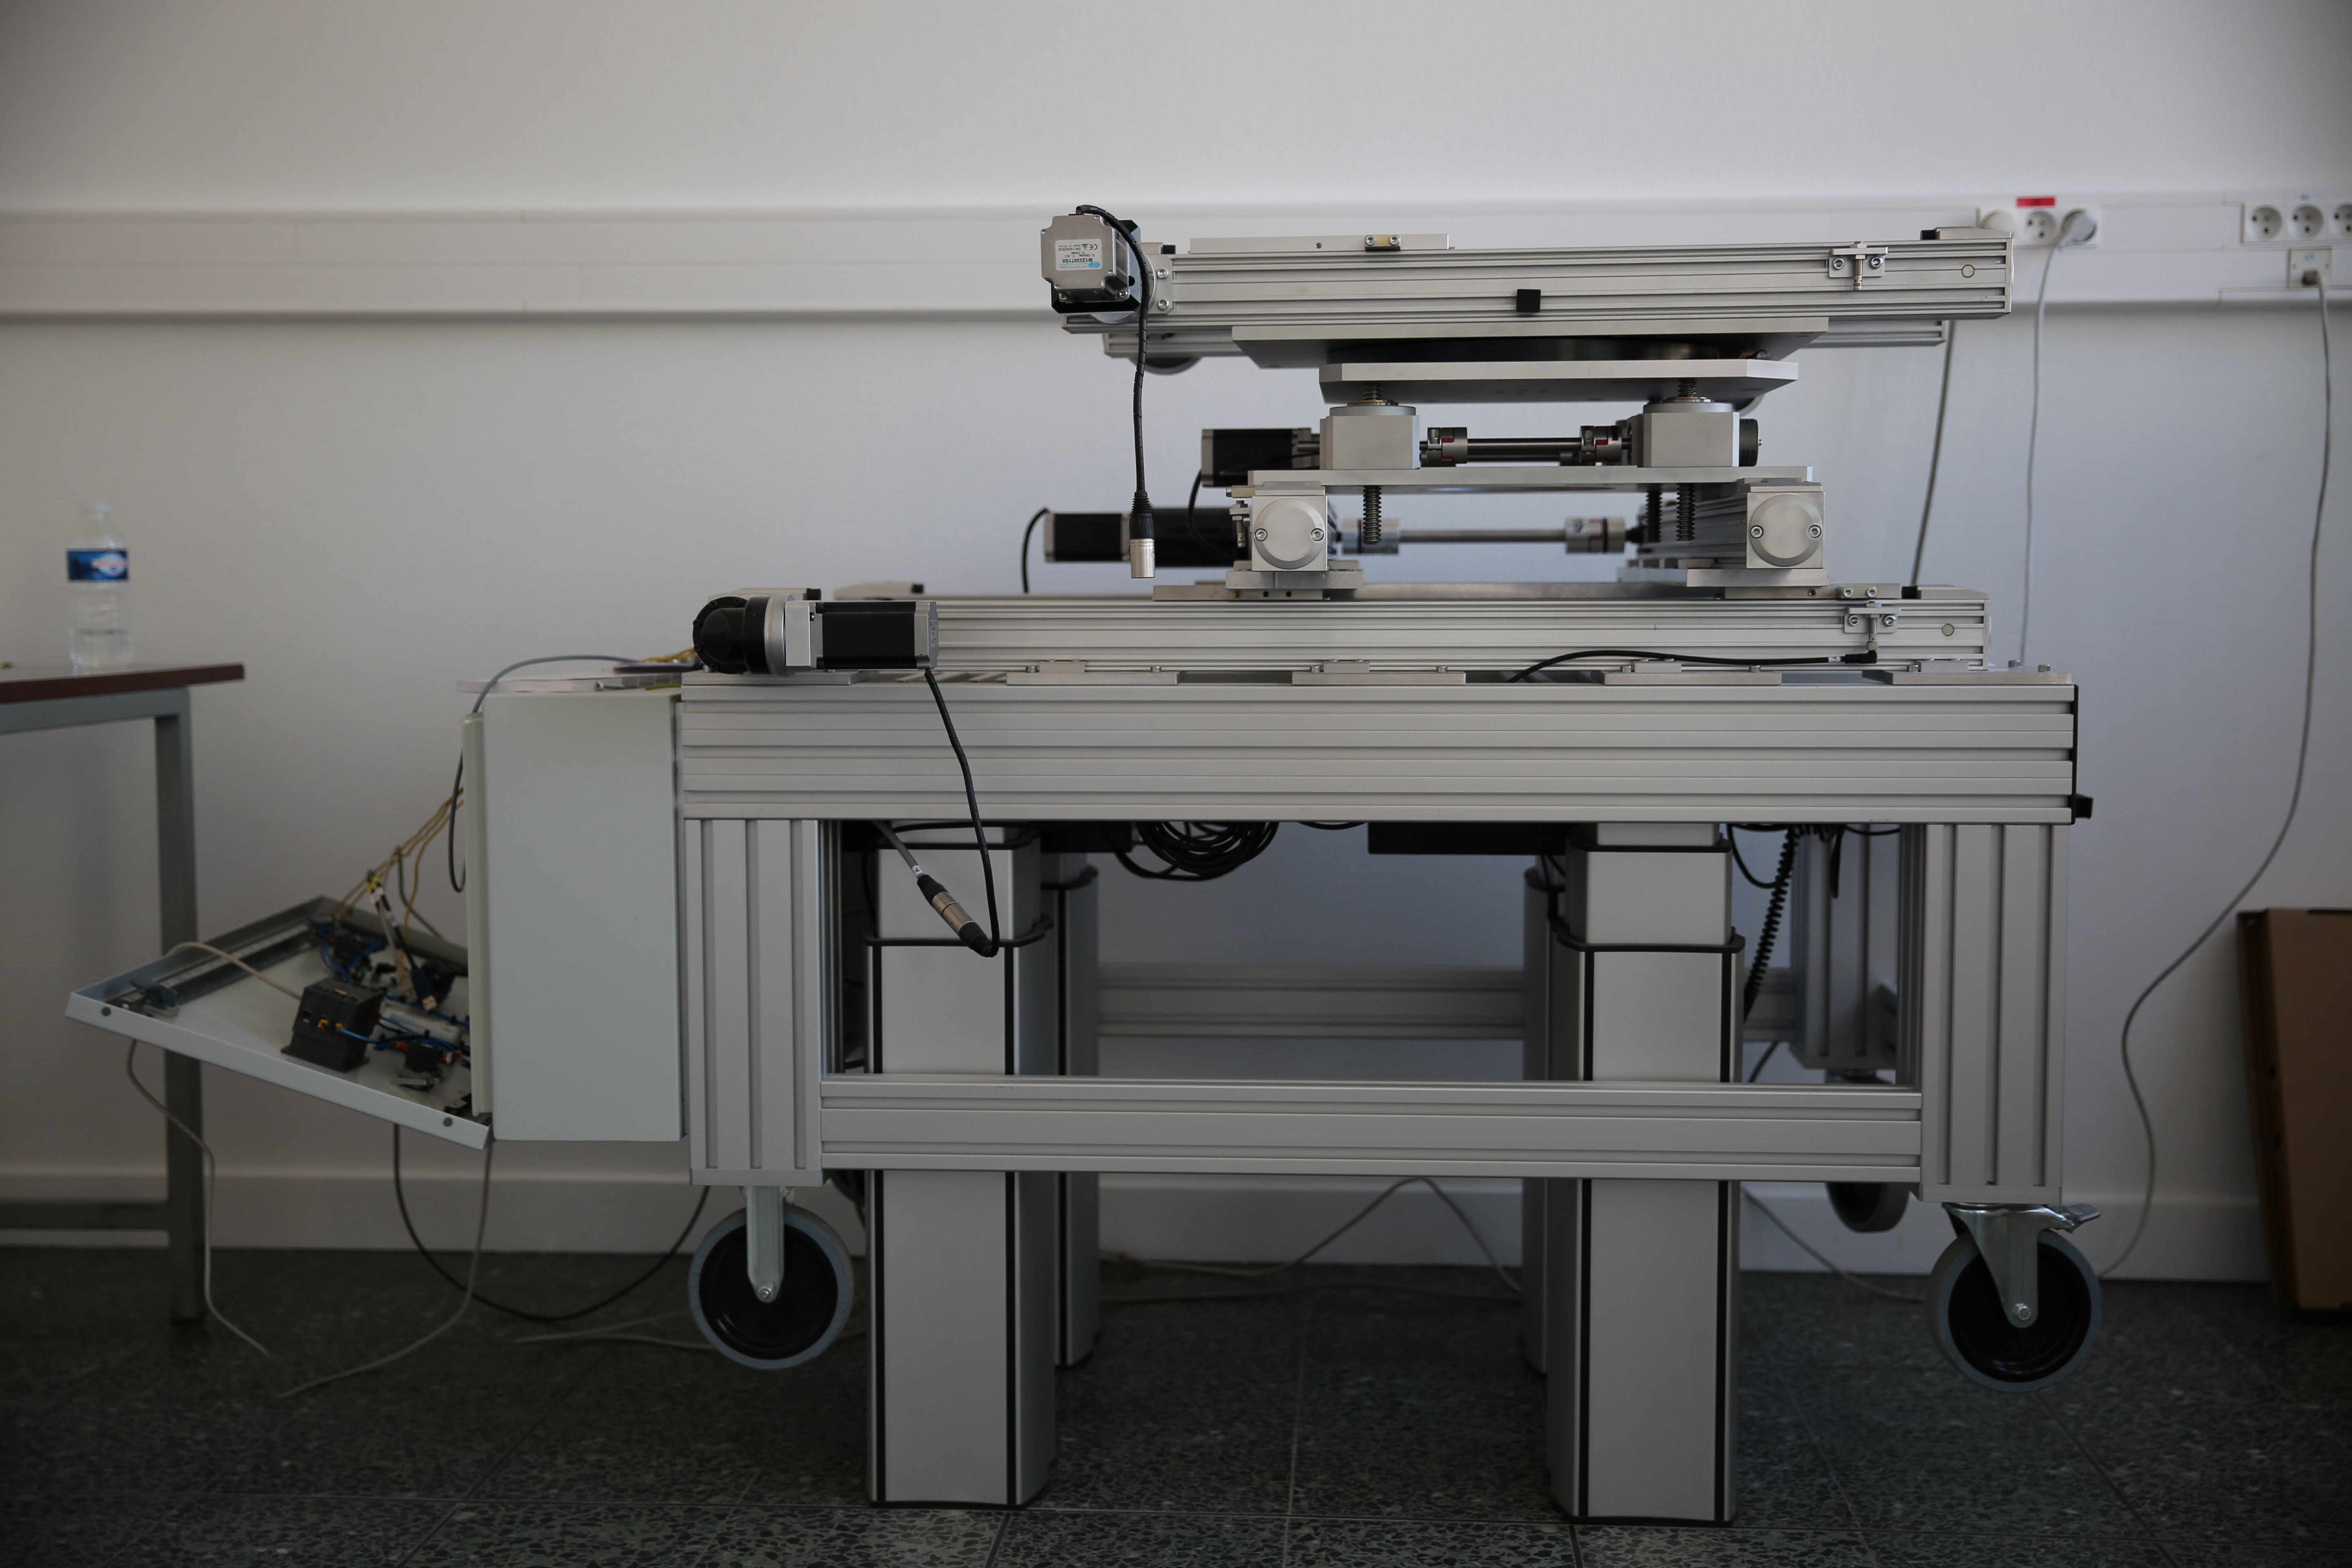
\includegraphics[width=0.8\textwidth]{03_GraphicFiles/chapter3_CLaRySproto/Mechanics/Table.JPG}
\caption{}
\label{chap3::fig::pictureTable}
\end{subfigure}
\caption{}
\label{chap3::fig::CameraIntegration}
\end{figure}

%%%%%%%%%%%%%%%%%%%%%%%%%%%%%%%%%%   CHARACTERIZATION MEASUREMENTS  %%%%%%%%%%%%%%%%%%%%%%%%%%%%%%%%%%%%%%%%%%%%

\section{Camera component characterization}\label{chap3::sec::charMeasurements}


%%%%%%%%%%%%%%%%%%%%%%%%%%%%%%%%%%   NEXT  %%%%%%%%%%%%%%%%%%%%%%%%%%%%%%%%%%%%%%%%%%%%

\section{Next steps and perspectives}\label{chap3::sec::Next}



%%%%%%%%%%%%%%%%%%%%%%%%%%%%%%%%%%%%%%%%%%%%%%%%% FROM PAPER SPECT %%%%%%%%%%%%%%%%%%%%%%%%%%%%%%%%%%%%%%%%%%%%%%%%% 
The Compton camera is composed of a scatterer part, which includes seven parallel planes of silicon detectors, 9$\times$9$\times$0.2~cm$^{3}$, with 1~cm distance between the centers of two neighboring planes, and an absorber, composed of BGO blocks of size 3.5$\times$3.5$\times$3.0~cm$^{3}$. 


The following requirements governed the choice of silicon as scattering material, and BGO as absorber~\parencite{Richard2012}:
\begin{itemize}
\item[-] optimizing the single Compton event probability, without escape of the Compton electron from the detector where it is created;
\item[-] minimizing the Doppler effect (especially important for low energy gamma rays);
\item[-] obtaining the best possible energy resolution in the scatterer;
\item[-] ensuring the best possible spatial resolution in the absorber, also thanks to the maximization of the photo-effect absorption with the highest $Z$ material.
\end{itemize}


%%%%%%%%%%%%%%%%%%%%%%%%%%%%%%%%%%%%%%%%%%%%%%%%% FROM PAPER HT %%%%%%%%%%%%%%%%%%%%%%%%%%%%%%%%%%%%%%%%%%%%%%%%% 

\clearpage
%\printbibliography[heading=subbibintoc]
